Quicksort is a divide and conquer comparison sorting algorithm, and has both a serial and parallel implementation. Serial quicksort is one of the most frequently used sorting algorithms, because of its simple implementation and high efficiency. The quicksort work by choosing a pivot, and then sorting the elements based on the pivot, creating new subsets. Each new subset is then sorted by pivot again, resulting in the creation of the final array. The quicksort can be described using the steps seen in \cref{tab:quicksort}.

\begin{center}
	\fbox{
		\begin{tabular}{p{40pt} p{220pt}}
			\textbf{Step 1} & Choose pivot element\\
			\textbf{Step 2} & Compare all elements with pivot \\
			\textbf{Step 3} & Split into 3 array; less than pivot, equal to pivot and greater than pivot \\
			\textbf{Step 4} & Recurse on each array
		\end{tabular}
	}
	\captionof{table}{Steps of Quicksort}
	\label{tab:quicksort}
\end{center} 

The first step is to choose the pivot, for which there are many strategies e.g. first element, last element, random element or median element. The choice of the pivot is the limiting factor of the quicksort, choosing the wrong pivot, increases the step and work complexity to $\mathcal{O}(n)$ and $\mathcal{O}(n^2)$ respectively. Then the pivot is chosen right the quicksort has a step complexity of $\mathcal{O}(log ~ n)$ and a work complexity of $\mathcal{O}(n~log~n)$, proving the choose of pivot is important. The second step is to compare all the elements with the pivot. The third step is to create three arrays, one containing all the numbers below the pivot, one with all numbers equal to the pivot and one with all numbers above the pivot. This is called the 3-way quicksort. The fourth and final step is to recurse on the above and below array, calling the quicksort again. An example of the quicksort, using last element as pivot is seen in \cref{fig:sort_quicksort}.

\begin{figure}[ht]
	\centering
	\fbox{
		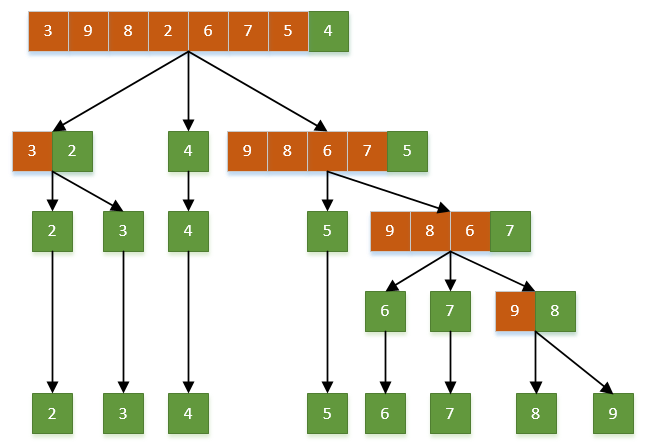
\includegraphics[width=0.7\textwidth]{figs/algorithm/sort_quicksort.png}}
	\caption{Example of the Quicksort, using last element pivot.}
	\label{fig:sort_quicksort}
\end{figure}  

One can implement the quicksort without recursion, but that is rather complicated, and is not as efficient as calling the quicksort with recursion. Not all languages and architectures support recursion, and this functionality was also first incorporated into the CUDA programming model in the 3.1 Toolkit \cite{cuda_3.1}.        